\PassOptionsToPackage{unicode=true}{hyperref} % options for packages loaded elsewhere
\PassOptionsToPackage{hyphens}{url}
\documentclass[12pt,ignorenonframetext,]{beamer}
\IfFileExists{pgfpages.sty}{\usepackage{pgfpages}}{}
\setbeamertemplate{caption}[numbered]
\setbeamertemplate{caption label separator}{: }
\setbeamercolor{caption name}{fg=normal text.fg}
\beamertemplatenavigationsymbolsempty
\usepackage{lmodern}
\usepackage{amssymb,amsmath}
\usepackage{ifxetex,ifluatex}
\usepackage{fixltx2e} % provides \textsubscript
\ifnum 0\ifxetex 1\fi\ifluatex 1\fi=0 % if pdftex
  \usepackage[T1]{fontenc}
  \usepackage[utf8]{inputenc}
\else % if luatex or xelatex
  \ifxetex
    \usepackage{mathspec}
  \else
    \usepackage{fontspec}
\fi
\defaultfontfeatures{Ligatures=TeX,Scale=MatchLowercase}







\fi

  \usetheme[]{metropolis}






% use upquote if available, for straight quotes in verbatim environments
\IfFileExists{upquote.sty}{\usepackage{upquote}}{}
% use microtype if available
\IfFileExists{microtype.sty}{%
  \usepackage{microtype}
  \UseMicrotypeSet[protrusion]{basicmath} % disable protrusion for tt fonts
}{}


\newif\ifbibliography


\hypersetup{
      pdftitle={A minimal example},
        pdfauthor={Matthias Vogelgesang},
          pdfborder={0 0 0},
    breaklinks=true}
%\urlstyle{same}  % Use monospace font for urls




  \usepackage{color}
  \usepackage{fancyvrb}
  \newcommand{\VerbBar}{|}
  \newcommand{\VERB}{\Verb[commandchars=\\\{\}]}
  \DefineVerbatimEnvironment{Highlighting}{Verbatim}{commandchars=\\\{\}}
  % Add ',fontsize=\small' for more characters per line
  \usepackage{framed}
  \definecolor{shadecolor}{RGB}{248,248,248}
  \newenvironment{Shaded}{\begin{snugshade}}{\end{snugshade}}
  \newcommand{\AlertTok}[1]{\textcolor[rgb]{0.94,0.16,0.16}{#1}}
  \newcommand{\AnnotationTok}[1]{\textcolor[rgb]{0.56,0.35,0.01}{\textbf{\textit{#1}}}}
  \newcommand{\AttributeTok}[1]{\textcolor[rgb]{0.77,0.63,0.00}{#1}}
  \newcommand{\BaseNTok}[1]{\textcolor[rgb]{0.00,0.00,0.81}{#1}}
  \newcommand{\BuiltInTok}[1]{#1}
  \newcommand{\CharTok}[1]{\textcolor[rgb]{0.31,0.60,0.02}{#1}}
  \newcommand{\CommentTok}[1]{\textcolor[rgb]{0.56,0.35,0.01}{\textit{#1}}}
  \newcommand{\CommentVarTok}[1]{\textcolor[rgb]{0.56,0.35,0.01}{\textbf{\textit{#1}}}}
  \newcommand{\ConstantTok}[1]{\textcolor[rgb]{0.00,0.00,0.00}{#1}}
  \newcommand{\ControlFlowTok}[1]{\textcolor[rgb]{0.13,0.29,0.53}{\textbf{#1}}}
  \newcommand{\DataTypeTok}[1]{\textcolor[rgb]{0.13,0.29,0.53}{#1}}
  \newcommand{\DecValTok}[1]{\textcolor[rgb]{0.00,0.00,0.81}{#1}}
  \newcommand{\DocumentationTok}[1]{\textcolor[rgb]{0.56,0.35,0.01}{\textbf{\textit{#1}}}}
  \newcommand{\ErrorTok}[1]{\textcolor[rgb]{0.64,0.00,0.00}{\textbf{#1}}}
  \newcommand{\ExtensionTok}[1]{#1}
  \newcommand{\FloatTok}[1]{\textcolor[rgb]{0.00,0.00,0.81}{#1}}
  \newcommand{\FunctionTok}[1]{\textcolor[rgb]{0.00,0.00,0.00}{#1}}
  \newcommand{\ImportTok}[1]{#1}
  \newcommand{\InformationTok}[1]{\textcolor[rgb]{0.56,0.35,0.01}{\textbf{\textit{#1}}}}
  \newcommand{\KeywordTok}[1]{\textcolor[rgb]{0.13,0.29,0.53}{\textbf{#1}}}
  \newcommand{\NormalTok}[1]{#1}
  \newcommand{\OperatorTok}[1]{\textcolor[rgb]{0.81,0.36,0.00}{\textbf{#1}}}
  \newcommand{\OtherTok}[1]{\textcolor[rgb]{0.56,0.35,0.01}{#1}}
  \newcommand{\PreprocessorTok}[1]{\textcolor[rgb]{0.56,0.35,0.01}{\textit{#1}}}
  \newcommand{\RegionMarkerTok}[1]{#1}
  \newcommand{\SpecialCharTok}[1]{\textcolor[rgb]{0.00,0.00,0.00}{#1}}
  \newcommand{\SpecialStringTok}[1]{\textcolor[rgb]{0.31,0.60,0.02}{#1}}
  \newcommand{\StringTok}[1]{\textcolor[rgb]{0.31,0.60,0.02}{#1}}
  \newcommand{\VariableTok}[1]{\textcolor[rgb]{0.00,0.00,0.00}{#1}}
  \newcommand{\VerbatimStringTok}[1]{\textcolor[rgb]{0.31,0.60,0.02}{#1}}
  \newcommand{\WarningTok}[1]{\textcolor[rgb]{0.56,0.35,0.01}{\textbf{\textit{#1}}}}

  \usepackage{longtable,booktabs}
  \usepackage{caption}
  % These lines are needed to make table captions work with longtable:
  \makeatletter
  \def\fnum@table{\tablename~\thetable}
  \makeatother

  \usepackage{graphicx,grffile}
  \makeatletter
  \def\maxwidth{\ifdim\Gin@nat@width>\linewidth\linewidth\else\Gin@nat@width\fi}
  \def\maxheight{\ifdim\Gin@nat@height>\textheight0.8\textheight\else\Gin@nat@height\fi}
  \makeatother
  % Scale images if necessary, so that they will not overflow the page
  % margins by default, and it is still possible to overwrite the defaults
  % using explicit options in \includegraphics[width, height, ...]{}
  \setkeys{Gin}{width=\maxwidth,height=\maxheight,keepaspectratio}

% Prevent slide breaks in the middle of a paragraph:
\widowpenalties 1 10000
\raggedbottom

  \AtBeginPart{
    \let\insertpartnumber\relax
    \let\partname\relax
    \frame{\partpage}
  }
  \AtBeginSection{
    \ifbibliography
    \else
      \let\insertsectionnumber\relax
      \let\sectionname\relax
      \frame{\sectionpage}
    \fi
  }
  \AtBeginSubsection{
    \let\insertsubsectionnumber\relax
    \let\subsectionname\relax
    \frame{\subsectionpage}
  }



\setlength{\parindent}{0pt}
\setlength{\parskip}{6pt plus 2pt minus 1pt}
\setlength{\emergencystretch}{3em}  % prevent overfull lines
\providecommand{\tightlist}{%
  \setlength{\itemsep}{0pt}\setlength{\parskip}{0pt}}

  \setcounter{secnumdepth}{0}



  \title[]{A minimal example}

  \subtitle{With a subtitle}

  \author[
        Matthias Vogelgesang
    ]{Matthias Vogelgesang}

  \institute[
    ]{
    Centre for Modern Beamer Themes
    }

\date[
      \today
  ]{
      \today
        }


\begin{document}

% Hide progress bar and footline on titlepage
  \begin{frame}[plain]
  \titlepage
  \end{frame}



\hypertarget{first-section}{%
\section{First Section}\label{first-section}}

\begin{frame}{First Frame}
\protect\hypertarget{first-frame}{}
Hello, world!
\end{frame}

\hypertarget{second-section}{%
\section{Second Section}\label{second-section}}

\begin{frame}{Second Frame}
\protect\hypertarget{second-frame}{}
\begin{block}{Bulleted Lists}
\protect\hypertarget{bulleted-lists}{}
\begin{itemize}
\tightlist
\item
  Element A
\item
  Element B

  \begin{itemize}
  \tightlist
  \item
    B.1
  \item
    B.2
  \end{itemize}
\item
  Element C
\end{itemize}
\end{block}
\end{frame}

\hypertarget{elements}{%
\section{Elements}\label{elements}}

\begin{frame}[fragile]{Typography}
\protect\hypertarget{typography}{}
\begin{verbatim}
The theme provides sensible defaults to
\emph{emphasize} text, \alert{accent} parts
or show \textbf{bold} results.

In Markdown, you can also use _emphasize_ and **bold**.
\end{verbatim}

\begin{center}becomes\end{center}

The theme provides sensible defaults to \emph{emphasize} text,
\alert{accent} parts or show \textbf{bold} results.

In Markdown, you can also use \emph{emphasize} and \textbf{bold}.
\end{frame}

\begin{frame}{Math}
\protect\hypertarget{math}{}
\begin{equation*}
    e = \lim_{n\to \infty} \left(1 + \frac{1}{n}\right)^n
\end{equation*}
\end{frame}

\begin{frame}[fragile]{R Figure Example}
\protect\hypertarget{r-figure-example}{}
The following code generates the plot on the next slide (taken from
\texttt{help(bxp)} and modified slightly):

\begin{Shaded}
\begin{Highlighting}[]
\FunctionTok{library}\NormalTok{(stats)}
\FunctionTok{set.seed}\NormalTok{(}\DecValTok{753}\NormalTok{)}
\NormalTok{bx.p }\OtherTok{\textless{}{-}} \FunctionTok{boxplot}\NormalTok{(}\FunctionTok{split}\NormalTok{(}\FunctionTok{rt}\NormalTok{(}\DecValTok{100}\NormalTok{, }\DecValTok{4}\NormalTok{),}
                      \FunctionTok{gl}\NormalTok{(}\DecValTok{5}\NormalTok{, }\DecValTok{20}\NormalTok{)), }\AttributeTok{plot=}\ConstantTok{FALSE}\NormalTok{)}
\FunctionTok{bxp}\NormalTok{(bx.p, }\AttributeTok{notch =} \ConstantTok{FALSE}\NormalTok{, }\AttributeTok{boxfill =} \StringTok{"lightblue"}\NormalTok{,}
    \AttributeTok{frame =} \ConstantTok{FALSE}\NormalTok{, }\AttributeTok{outl =} \ConstantTok{TRUE}\NormalTok{,}
    \AttributeTok{main =} \StringTok{"Example from help(bxp)"}\NormalTok{)}
\end{Highlighting}
\end{Shaded}
\end{frame}

\begin{frame}{R Figure Example}
\protect\hypertarget{r-figure-example-1}{}
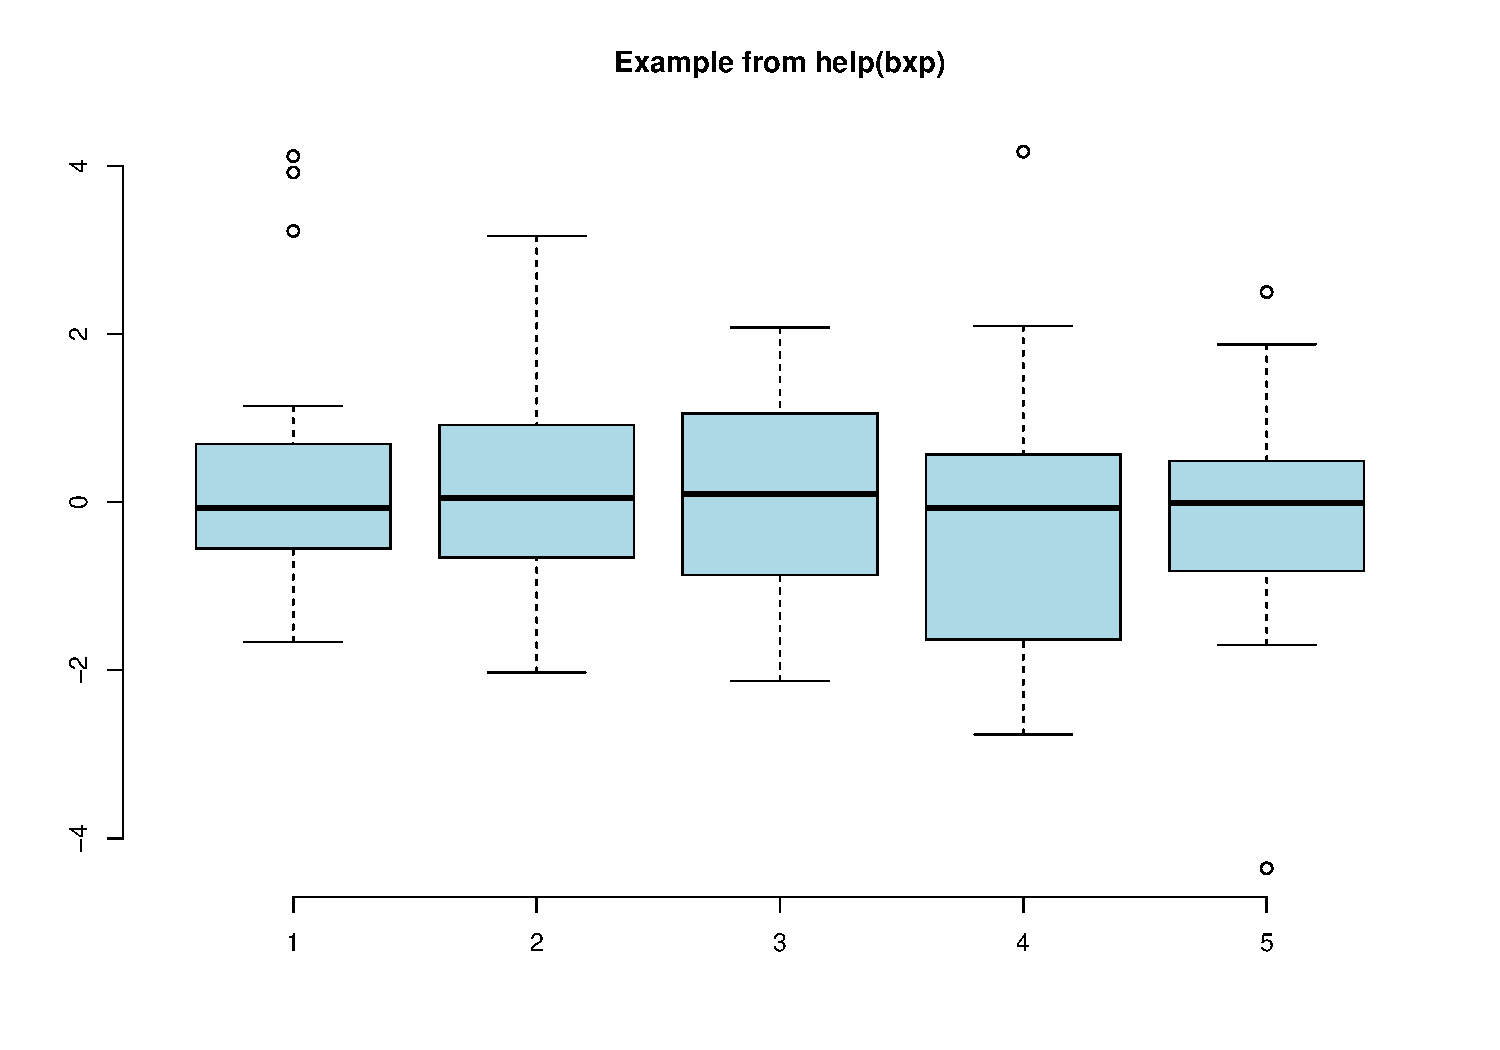
\includegraphics{myslides_files/figure-beamer/pressureFig-1.pdf}
\end{frame}

\begin{frame}[fragile]{R Table Example}
\protect\hypertarget{r-table-example}{}
A simple \texttt{knitr::kable} example:

\begin{Shaded}
\begin{Highlighting}[]
\NormalTok{knitr}\SpecialCharTok{::}\FunctionTok{kable}\NormalTok{(mtcars[}\DecValTok{1}\SpecialCharTok{:}\DecValTok{5}\NormalTok{, }\DecValTok{1}\SpecialCharTok{:}\DecValTok{8}\NormalTok{],}
             \AttributeTok{caption=}\StringTok{"(Parts of) the mtcars dataset"}\NormalTok{)}
\end{Highlighting}
\end{Shaded}

\begin{longtable}[]{@{}lrrrrrrrr@{}}
\caption{(Parts of) the mtcars dataset}\tabularnewline
\toprule
& mpg & cyl & disp & hp & drat & wt & qsec & vs\tabularnewline
\midrule
\endfirsthead
\toprule
& mpg & cyl & disp & hp & drat & wt & qsec & vs\tabularnewline
\midrule
\endhead
Mazda RX4 & 21.0 & 6 & 160 & 110 & 3.90 & 2.620 & 16.46 &
0\tabularnewline
Mazda RX4 Wag & 21.0 & 6 & 160 & 110 & 3.90 & 2.875 & 17.02 &
0\tabularnewline
Datsun 710 & 22.8 & 4 & 108 & 93 & 3.85 & 2.320 & 18.61 &
1\tabularnewline
Hornet 4 Drive & 21.4 & 6 & 258 & 110 & 3.08 & 3.215 & 19.44 &
1\tabularnewline
Hornet Sportabout & 18.7 & 8 & 360 & 175 & 3.15 & 3.440 & 17.02 &
0\tabularnewline
\bottomrule
\end{longtable}
\end{frame}

\begin{frame}{Resources}
\protect\hypertarget{resources}{}
\begin{block}{For more information:}
\protect\hypertarget{for-more-information}{}
\begin{itemize}
\tightlist
\item
  See the \href{https://github.com/matze/mtheme}{Metropolis repository}
  for more on Metropolis
\item
  See the \href{https://github.com/rstudio/rmarkdown}{RMarkdown
  repository} for more on RMarkdown
\item
  See the \href{https://github.com/eddelbuettel/binb}{binb repository}
  for more on binb
\item
  See the \href{https://github.com/eddelbuettel/binb/vignettes}{binb
  vignettes} for more examples.
\end{itemize}
\end{block}
\end{frame}




\end{document}
